\chapter{Introdução}

\section{(Pré) História}

Tudo começa na floresta, em meio à umidade que persiste entre dezembro e
junho, durante um inverno qualquer no início da década de 1990. Contam
que o episódio se passou nas cabeceiras do rio Caru, no igarapé
Mão de Onça, mas bem poderia ter se dado pelo Pindaré, Turiaçu ou até
mesmo em algum afluente do longínquo rio Gurupi. Pakwa'ĩa ainda era uma
menina, com menos de dez anos, e se lembra de quando sua mãe, Panyxĩa, e
seu pai, Kamara, (pois, apesar de ser \emph{awa}/``humano'', é assim que
os outros o chamam: ``estrangeiro''/\emph{kamará}) por causa da chuva ou
de descuido, deixaram apagar o toco de madeira em brasa que carregavam
em suas andanças. Este tição de fogo (\emph{jamakaipẽ}), feito com
madeira de sapucaia, garantia o preparo da comida, aquecia os corpos e
espantava os \emph{ajỹ} (seres"-espectros da floresta que matam ou fazem
adoecer as pessoas) durante a noite. Formavam uma família pequena,
composta pelo casal e seus dois filhos: um menino de colo, Juma'ã --- hoje
um homem belo e forte ---, e a mais velha, Pakwa'ĩa, hoje mãe de três
meninas e que agora me conta esta história.

Àquela época, a família de Pakwa'ĩa vivia nas matas do Caru,
\emph{haka'a} (``minha mata''), caçando macaco capelão (\emph{Alouatta
belzebul}) e comendo mel. Também comiam bacaba, pequi e babaçu; caçavam
queixadas, caititus, antas e diversos macacos, além de comerem muito
jabotis, jabotas, capiningas, cotias e pacas, dentre tantos outros
animais que aqui encontraremos. Panyxĩa e Kamara sabiam que alguns de
seus parentes próximos e os afins, distantes em geral, estavam morrendo
em virtude do ``catarro'' (\emph{ju'u}, ``tosse'') trazido pelos
\emph{brancos}, os \emph{karai}. Enquanto alguns fugiram apavorados,
outros, sem muita opção ou movidos por um fio de esperança, procuraram
fazer contato. Kamara ainda estava receoso sobre esse encontro e
preferiu não aparecer com sua família, mesmo com todas as ofertas de
objetos e outros itens que ele encontrava nos locais onde os
\emph{brancos} iam procurá"-lo. Segundo Kamara, foram os Guajá que
apareceram aos \emph{brancos} e se quisessem nunca teriam feito contato. Algumas famílias morreram quando fugiam dos \emph{karai}, como
o próprio irmão de Kamara; outras se separaram, enquanto outras ainda
estão sem contato --- conta"-me uma Pakwa'ĩa muito interessada nos
\emph{awa mihua}, essa ``gente do mato'' que até hoje vive isolada.

O tal tição se apagara, e a família se viu sem o seu fogo,
\emph{tata}, e da mesma maneira que ocorreu aos Yuquí/Sirionó da Bolívia
(Holmberg, 1969; Balée, 1991), os Parakanã ocidentais (Fausto, 2001),
dentre tantos outros povos do mundo, os Guajá em seus anos de fuga
perderam a arte de fazer fogo. Porém, mesmo não sabendo produzi"-lo,
cultivavam a brasa mantendo o tição vivo aonde quer que fossem. Isto era
suficiente para moquear as carnes que chegavam às aldeias, cozinhar o
fruto de \emph{pinawã} (bacaba) ou a macia carne do peixe elétrico
poraquê (\emph{myrakya}) em embalagens confeccionadas com folhas frescas
da palmeira \emph{jahara} (açaí), pois também não dominavam a arte de
produção da cerâmica. O estoque de carne moqueada ainda era suficiente
para alguns dias, porém quando este terminasse a pequena Pakwa'ĩa e sua
família poderiam passar momentos difíceis. Sem ter como produzir fogo,
Kamara se lembrou de um antigo local onde passara junto com outros
grupos uma temporada de verão. Rememorou haver perto de lá uma roça de
milho (\emph{waxia}), muito provavelmente plantada pelos \emph{karai}
(não indígenas), e, embora não se interessasse em consumir aquele
alimento, sabia que os \emph{karai} gostavam muito dele, e certamente
haveria \emph{brancos} por perto.

Muitos chamariam a aldeia em que esta família estava de ``acampamento'',
seja porque as casas eram tapiris (\emph{tapa'ĩ}) --- que consistiam em
algumas palhas amarradas em troncos de árvores ou em alguma estrutura de
paus ---, seja por não haver roças perto, assemelhadas a um típico
acampamento de caça, pelo que muitas vezes a aldeia durava menos do que
uma estação. Lembro aqui que seus vizinhos --- e inimigos históricos ---
Ka'apor costumavam dizer que os Guajá viviam como ``macacos'', comendo
frutos, e que essas aldeias não passavam de um ``amontoado de casas de
palha de açaí ou pindó sobre paus dobrados ou partidos a pauladas porque
eles não têm terçados'' (Ribeiro, 1996, p. 262). Trata"-se de uma
atualização típica de uma famosa relação ameríndia, em que povos com
alguma agricultura costumam hostilizar seus vizinhos que não se
interessam pelo plantio. ``Macacos'', não por coincidência, era o termo
empregado pelos Tukano, do Alto Rio Negro, para se referir a seus
vizinhos do grupo linguístico Makú (Silverwood-Cope, 1990). Esta era a
aldeia da família de Pakwa'ĩa ou seu \emph{haripa} (``minha casa''),
como dizem os Guajá. Se a literatura antropológica definiu este tipo de
ocupação como ``acampamento'', ``retiro de caça'' e coisas do gênero,
Pakwa'ĩa a apresentou a mim como ``sua casa''.

Embora não conhecessem a agricultura e não erguessem aldeias fixas,
enganam"-se os que pensam que o nomadismo Guajá fosse algum tipo de
``mobilidade pioneira'', sempre à procura de novos e inexplorados sítios
para ocupar um novo manancial de caça e coleta. Ao contrário, quanto
mais conhecido o espaço, mais preferível era para permanecer.
\emph{Harakwaha} seria a objetivação da ideia de ``território''. Podemos
traduzi"-lo como ``meu domínio'' ou ``meu lugar'', e se trata da área de
um grupo, que poderia variar de uma pequena família, como a de Pakwa'ĩa,
a até 30 pessoas que por algum motivo estivessem juntas. O
\emph{harakwaha}, por sua vez, é um conjunto de sítios, cada um com uma
história, boa ou ruim, para recordar: antigas aldeias, vestígios de
animais caçados, restos de ossos humanos que devem ser evitados,
``aquela árvore de maçaranduba onde matei dois veados\ldots{}'' assim a
memória é desencadeada pela relação com o espaço (como veremos no
capítulo 2).

Um desses locais que outrora conhecera e agora jazia abandonado era a roça
de milho que Kamara decidiu observar, a fim de procurar a casa de algum
\emph{branco} e conseguir novamente fogo para sua brasa. Receoso em
levar junto sua mulher, filha e o pequeno Juma'ã, ainda de colo, o homem
decidiu deixá"-los bem instalados na pequena aldeia perto de um açaizal,
recém"-construída com a ajuda de seu irmão, que neste momento já havia
partido para outra região e nunca mais aparecera. A aldeia, além de um
tapiri e um moquém, possuía uma tímida clareira e estava no alto de um
monte com um igarapé logo abaixo, cujas águas sua esposa, Panyxĩa, usava
para cuidar das crianças, na expectativa de que seu marido voltasse com
fogo. Comiam ali bacaba (\emph{pinawã}), babaçú (\emph{hwa'ĩ}) e o
restante da carne de um macaco prego moqueado (\emph{ka'i}). Enquanto
isso Kamara caminhava pelas serras, \emph{wytyra}, que compõem as
florestas da bacia do rio Pindaré. Embora os Guajá os tivessem evitado
durante um longo período de tempo, os \emph{brancos} nunca estiveram
distantes. A região pré"-amazônica, além de ser densamente povoada,
recebeu sistematicamente colonos oriundos de vários estados do nordeste
do Brasil, com uma migração intensa a partir da segunda metade da década
de 1960. Os Guajá, cujo problema até então consistia nos conflitos
intestinos com os Ka'apor e Tenetehara, passaram então a conviver com
uma ameaça ainda maior.

Kamara, que na época estava com os seus 40 anos, sabia de tudo isso, e
provavelmente seu pai tenha vivido os mesmos problemas: pelo oeste e
parte do sul de sua área, os \emph{karai} (não indígenas) e os Tenetehara, e a leste e norte os outros \emph{kamara} (indígenas
Ka'apor e Tenetehara). Como sua família necessitava de fogo e os outros
\emph{awa} (gente) estavam a alguns dias de caminhada, resolveu ir ao
encontro do grupo de \emph{brancos} que, ele sabia, morava perto daquela
roça de milho. Da descrição do encontro em si não tenho muitos detalhes,
até porque, disse"-me Pakwa'ĩa, o que ela sabe está em sua lembrança de
uma menina de sete anos. Hoje eu sei que esse antigo morador se chamava
``Seu Olímpio'' e vivia em um dos limites da Terra Indígena. Kamara
conseguiu o fogo de que precisava, na forma de um isqueiro, e ainda
recebeu desse Seu Olímpio uma pequena panela e uma faca bem gasta, porém
com algum corte. Alguns anos depois, em 1997, a família de Kamara viria
a ser oficialmente contatada pela Fundação Nacional do Índio (\textsc{funai}),
ironicamente após o órgão ter decidido extinguir a Frente de Atração por
alegar não haver mais ``Guajás isolados''.

Estas são as pessoas pelas quais este livro se interessa. Elas fazem
parte de um coletivo ameríndio que conseguiu resistir aos encontros com
o \emph{Brasil}. Porém, nos últimos anos, um pequeno e último
contingente que vivia sem contato oficial vem aparecendo por não ter
mais para onde fugir.

\section{Caminhando com os Guajá: sobre o trajeto e a pesquisa}

Este livro está baseado em um período de 13 meses de trabalho de campo,
em viagens a três diferentes aldeias ocorridas entre os anos de 2007 e
2013. Em algumas das viagens eu permanecia cerca de três meses no campo,
enquanto nas últimas, já no período de pós"-doutorado, as incursões
duravam por volta de um mês. As aldeias onde a pesquisa se desenvolveu
(Juriti, Tiracambu, e Awá)
%manter essa referência no meio do texto?
 situam"-se nas Terras Indígenas (\textsc{ti}) Carú e Awá, e uma
distância de 150 km separa as pessoas da \textsc{ti} Carú e Awá, embora estas áreas
sejam contíguas. Se historicamente esses dois conjuntos
populacionais experimentam pouco contato, muitas pessoas que hoje se
encontram separadas viveram juntas no ``tempo do mato'' (\emph{ka'ape
mỹna}, ``antigamente na floresta'').\footnote{Este é o caso da família da
  matriarca Amỹ Paranawãja da aldeia Tiracambu, cujos filhos são
  germanos (\emph{hapihiara}) de outros das aldeias Awá e Juriti.} As
antigas Frentes de Atração --- como é costume até hoje nas atuais Frentes
de Proteção --- recrutavam indígenas para ajudar como intérpretes nos
contatos. Um dos chamarizes para os homens que auxiliavam a \textsc{funai} era a
possibilidade de conseguirem novas esposas nos contatos. Tais encontros
colaboraram diretamente para uma redistribuição das pessoas nas atuais
quatro aldeias, quando casais se formavam por meio desse trânsito. Na
busca por parentes do mato, homens, casais e mesmo famílias inteiras se
mudavam para as novas aldeias que surgiam (como Juriti e Tiracambu), e a
partir daí ocorriam novas configurações políticas. O resultado podemos
ver hoje: parentes entre si espalhados por todas as aldeias, seja por
relações anteriores, seja por essa reengenharia particular posterior ao
contato.

%\textbf{Foto da aldeia Awá}
%\begin{figure}[H]
%\centering
 % 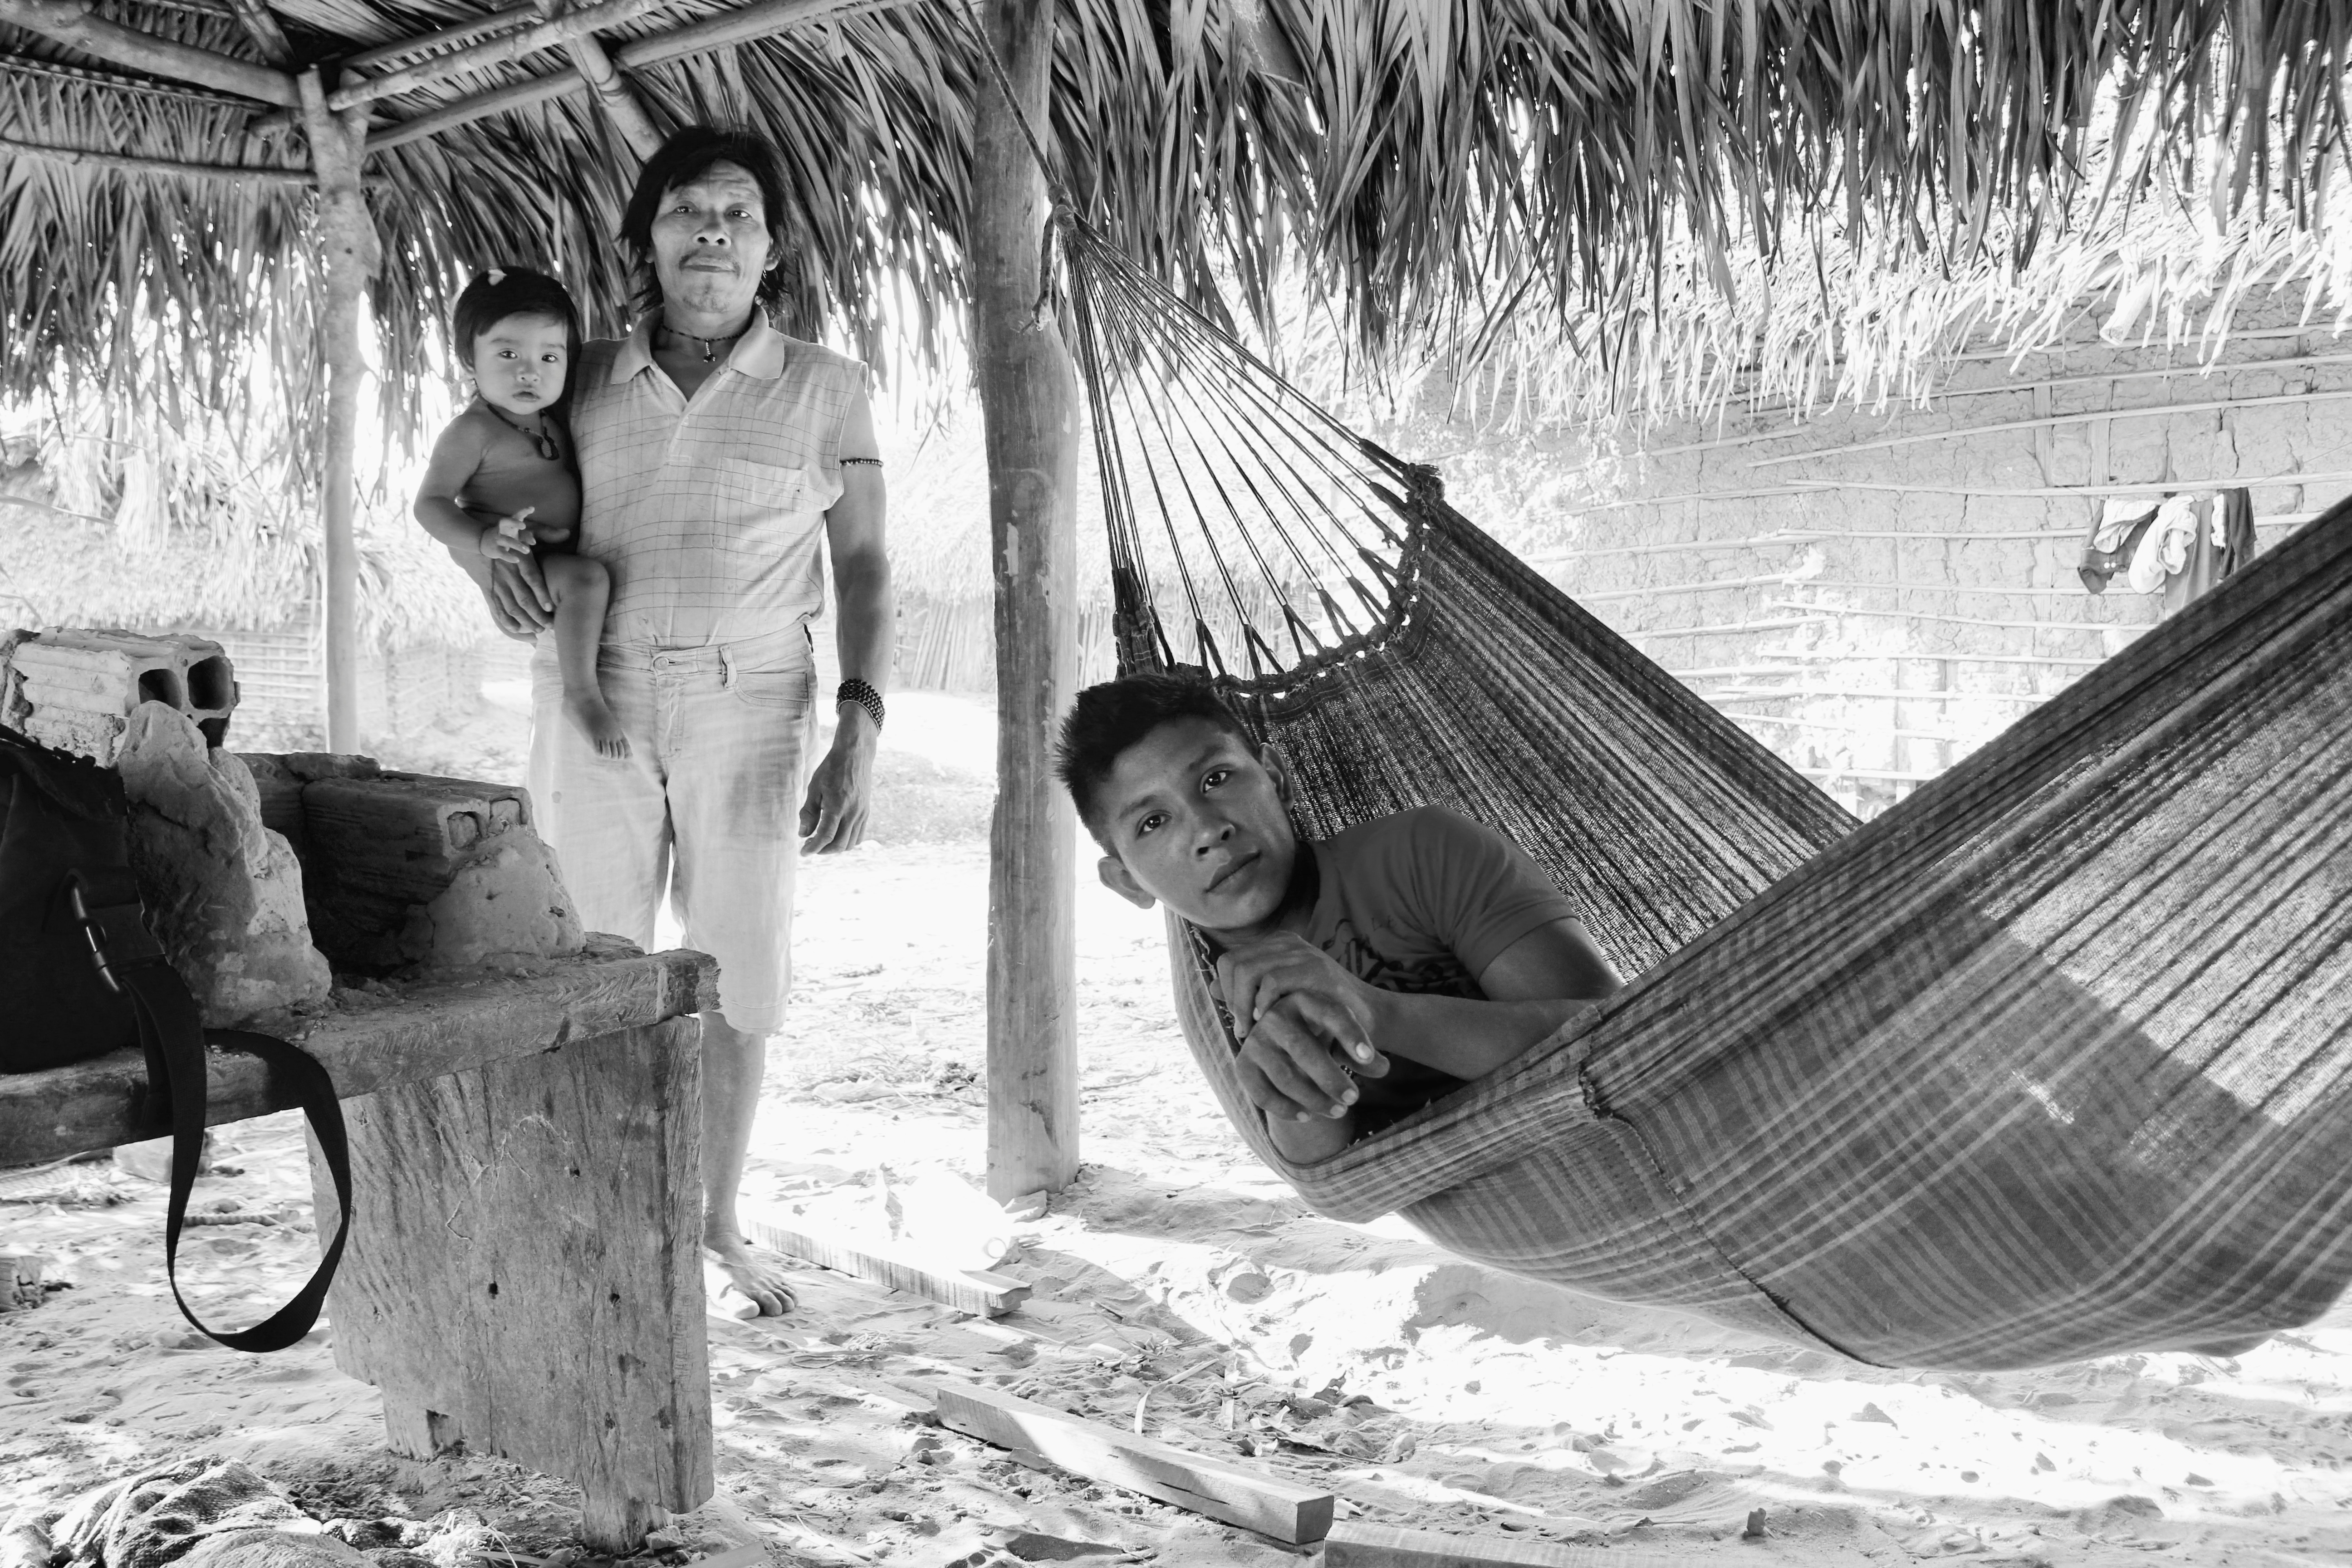
\includegraphics[width=\textwidth]{./imgs/IMG_4983}
%\caption{Hajkaramykỹa com sua filha de colo junto a Petua, deitado na rede (Aldeia Awá, 2014).}
%\end{figure}

Os Guajá são matéria de meus interesses de estudo desde os anos de
mestrado, e a pesquisa etnográfica propriamente foi iniciada durante o
trabalho de doutorado na Universidade de São Paulo (\textsc{usp}). Nesta época
pude realizar uma investigação mais geral sobre o estudo das práticas de
conhecimento relativas aos animais e à caça entre os Guajá, em diálogo
com a teoria antropológica amazônica recente. Para tanto me interessei
pelos regimes de subjetivação e sistemas de ação, particularmente em
objetos de análise, tais como parentesco/pessoa, caça/território e
cosmologia. Tais abordagens desdobraram a investigação em um tema
tributário --- desenvolvido durante meu pós"-doutorado na Universidade
Estadual de Campinas (Unicamp) --- que pode ser definido como a tentativa
de formulação de uma \emph{teoria etnográfica da caça guajá}. Em linhas
gerais, a forma como tais pessoas percebem e executam as atividades de
caça, por ocupar um lugar proeminente na socialidade humana, nos
informaria sobre a maneira como o próprio mundo e suas relações são
compostos. Esta pesquisa foi um passo na tentativa de pensar a caça e os
conhecimentos que a cercam, pelas vias da percepção e da relação entre
caça e cosmologia. Tal preferência teórica não foi apenas uma opção
pessoal, mas procurou seguir as pistas que os próprios Guajá sugeriam ao
definirem a atividade de caça como arte do ``escutar'', do ``imitar'', do
``enganar'', a partir de uma dimensão acústica da caça.

Ao lado disso, um ponto a ser lembrado é que talvez seja impossível para
nós, antropólogos, trabalharmos com qualquer povo indígena no Brasil
atual sem nos envolvermos com os problemas e soluções que afetam
diretamente suas relações territoriais e sociocosmológicas, algo próximo
àquilo que Ramos (1990) denominou \emph{Ethnology Brazilian Style}.
Uma combinação entre pesquisa acadêmica e envolvimento político, à
revelia dos próprios anseios dos etnólogos. A relação de confiança entre
antropólogos e as comunidades nas quais estamos inseridos, sobretudo no
Brasil contemporâneo quando os povos indígenas e seus direitos continuam
a experimentar entraves, tem como resultado muitas vezes o paralelismo
entre a ação (indigenista) e a reflexão (antropológica). O caso de minha
pesquisa de pós"-doutorado finalizada em 2014, na qual me interesso pela
relação entre caça e sonoridades, pareceu"-me prototípico neste tópico.
Se meus interesses iniciais visavam ao aprofundamento de questões
teóricas e etnográficas que mereciam ser mais bem examinadas, sobretudo
o que chamei de ``dimensão acústica da caça'', essas mesmas questões
acabaram por revelar --- dentro do contexto de rápida transformação
ambiental por que passam os territórios guajá --- detalhes sobre a
mudança de vida dessas populações. A relação entre ``conhecimento'' e
``acústica'' para os Guajá é direta, e o processo de degradação ambiental
é lembrado como repleto de ``barulho'' (\emph{iau}), produzindo"-se
desequilíbrio ecológico (nos termos também de uma ``ecologia acústica'',
cf. Feld, 1994) em um mundo em que a ideia (e a palavra) ``escutar''
(\emph{nũ}) é sinônimo de ``entender/conhecer'' (\emph{idem}). Um ``saber
ouvir'', em todas as suas dimensões, é uma importante forma de
conhecimento para este povo. Os grupos chamados \emph{mihua}, os
``isolados'', como veremos neste livro, por sua vez viveriam uma vida
silenciosa na qual sua sobrevivência dependeria de não serem vistos ou
ouvidos.

Mesmo contatados e com seus territórios homologados, os Guajá têm
experimentado pressões de grileiros, pecuaristas, pequenos agricultores,
madeireiros e narcotraficantes que ocupam suas terras --- o último
resquício de floresta no estado do Maranhão. Pessoas de diferentes
aldeias apontam de maneira muito direta os efeitos do desmatamento e da
existência de uma ferrovia na borda de uma de suas terras. Os Guajá
empreendem uma interessante crítica à poluição ambiental e sonora que se
instalou em seu horizonte lembrando o barulho que espanta os animais em
geral (e os de caça, especificamente) e assusta suas crianças; o
trepidar da terra com a passagem do trem; a poeira e poluentes diversos
que escapam das cargas de minério de ferro perto dos rios e floresta no
decorrer da ferrovia que se espalha ao longo da \textsc{ti} Caru; a chegada cada
vez mais frequente de criadores de gado, madeireiros e pequenos
caçadores para perto dos acessos da \textsc{ti}, o que faz as pessoas se
perguntarem até quando as crianças se alimentarão de maneira farta com
``comida de gente'' (\emph{awa nimi'ũa}). ``Os animais se foram!'' e
``Meus filhos estão com fome!'' são lamentos cada vez mais comuns
ouvidos em aldeias como Juriti, Tiracambu e Awá. Um dos maiores desafios
teóricos que me foi imposto pela etnografia foi conjugar os esforços de
pesquisa à delicada situação em que se encontravam (e ainda se
encontram) meus interlocutores.

Balancear a pesquisa frente à situação política dos Guajá com as três
Terras Indígenas onde vivem sendo incluídas no grupo das mais desmatadas
da Amazônia Legal (Greenpeace, 2014) fez com que eu me envolvesse de
forma colaborativa com organizações como a \textsc{ong} inglesa Survival
International e, de maneira mais pontual, com o Conselho Indigenista
Missionário (\textsc{cimi}) e a \textsc{ong} ambientalista Greenpeace. A própria
Coordenação Geral de Índios Isolados e Recém"-Contatados (\textsc{cgiirc}) da
\textsc{funai}, pela urgência da situação, me convidou junto com a colega e
linguista Marina Magalhães (docente do departamento de linguística da
\textsc{u}n\textsc{b} e estudiosa da língua Guajá) para facilitarmos junto às comunidades
um programa de apoio permanente aos Guajá, batizado de ``Programa Awá'',
cuja primeira grande ação foi a (até agora) bem"-sucedida desintrusão da
\textsc{ti} Awá durante o primeiro semestre de 2014. Neste momento está em curso
a criação da primeira associação indígena Guajá na esperança de que as
comunidades ganhem autonomia e desenvolvam seus próprios projetos.

\section{O Livro}

O conteúdo do livro discute as formas de relação de pessoas que se
definem como \emph{awa} (``humanos'') com o seu mundo, articulando"-se os
campos do parentesco, caça e cosmologia. Em diálogo com boa parte da
literatura Tupi (clássica e contemporânea) e com um escopo mais amplo de
autores e etnografias, o trabalho pretende ser uma contribuição
etnográfica e teórica para a etnologia das terras baixas sul"-americanas.

Os temas aparecem articulados da segunite forma:

No capítulo 1, apresento a história recente permeada pelos
contatos, fugas, mortes na floresta e recomeços em novas aldeias.
Trata"-se de histórias que os Guajá não nos deixam esquecer e que são
constantemente rememoradas quando as pessoas falam de si, da família ou
dos amigos. O objetivo deste capítulo é discutir esses caminhos de fugas
e transformações que marcaram a vida das pessoas em um passado recente.

O capítulo 2 se dedica às formas de relação no espaço e como os
Guajá concebem seu território, com destaque para a noção de
\emph{harakwaha}. Neste capítulo faço a passagem da geografia para a
cosmografia, em que se apresenta a divisão do mundo em diversos
patamares e como tais níveis de existência se articulam.

No capítulo 3, faço uma descrição dos componentes que marcam a
``humanidade'' (\emph{awatea}, ``gente de verdade''), as concepções sobre
o corpo e a vitalidade, além de uma antropologia interessada nas
alegrias, tristezas, sonhos, onomástica, comensalidade, enfim, elementos
que compõem a própria existência.

No capítulo 4, mostro as chamadas \emph{relações de alteridade}
com outros povos indígenas, além de apresentar as diferenças
experimentadas entre as pessoas das diversas comunidades Guajá. O
objetivo do capítulo é refletir criticamente sobre as formas de relações
humanas apontando para a ideia de que não podemos falar em uma
``totalidade'' Awá"-Guajá, ou em algo como um \emph{grupo} que se veja
como unidade. Veremos que a própria ideia de \emph{grupo} ou
\emph{coletivo} representada no pronome exclusivo \emph{aria}, ``nós'' ---
como é confirmado por tantos casos ameríndios --- variará de acordo com o
espectro de relações que as pessoas travam entre si.

O capítulo 5 faz uma descrição do sistema de aliança, com
algumas observações sobre o parentesco Guajá de uma maneira geral. Neste
capítulo apresento a hipótese de que o casamento é uma relação de
``criação'', pensada como uma relação \emph{riku}, tal como outras
relações no mundo.

No capítulo 6, articulo a ideia de \emph{riku} com outras relações homólogas, mas que não seriam
propriamente do plano do parentesco humano. Neste capítulo procuro
dialogar com as ideias de ``donos'' e ``criaturas'', tal como discutidas em
outros contextos amazônicos.

Os capítulos 7 e 8 são uma descrição das atividades de caça
que, além de articularem alguns temas dos capítulos anteriores, sugerem
que a caça se relaciona não só com a ecologia, mas também com o
parentesco, a guerra e a cosmologia. A partir da apresentação das
técnicas e relações entre caçadores e presas, os capítulos discutem o
engajamento particular dos Guajá em tal atividade, a caça feminina, a
parafernália de caça e as relações humano"-animais.

No capítulo 9, esboço a relação dos Guajá com os
\emph{karawara}, seres que já terão aparecido em vários momentos do
livro. Os \emph{karawara} podem ser pensados como subjetividades que
povoam os patamares celestes e são, ao mesmo tempo, o destino \emph{post
mortem} dos humanos. O capítulo apresenta a complexidade desses seres
que mobilizam uma ontologia própria, relacionando de maneira muito
original a caça e o xamanismo. Neste capítulo indico como a
cosmologia está intimamente ligada às atividades de caça, sendo os
\emph{karawara}, ao mesmo tempo, caçadores e xamãs magníficos.

\section{Etnografia}

Durante o livro apresentarei experiências que me permitiram compreender
aos poucos os conhecimentos e o mundo Guajá. São histórias vividas por
eles, outras que me contaram sobre diversas pessoas, e outras tantas que
experimentamos juntos em nossa convivência, traduzidas aqui não sem uma
dose de especulação baseada na observação. Em muitas ocasiões me sentia
o ``nativo'', pois por diversas vezes, e não foram poucas, eles é que me
sabatinavam a respeito do meu mundo. Num primeiro momento, essa intensa
curiosidade me provocava certa decepção: a de achar que não estava
conseguindo conhecê"-los, pois só queriam saber de mim, e eu pensava não
estar aprendendo nada sobre \emph{eles}. No entanto, isso fez com que
nos aproximássemos, tanto pela confiança mútua que impera nesses jogos
de perguntas e respostas, quanto por conseguir perceber quão desgastante
é ser entrevistado sobre temas tão diferentes que aparecem em conversas
quando nos interessamos por tudo aquilo relacionado ao mundo de outra
pessoa.

Das desventuras de campo que experimentam os etnógrafos, pude viver
diversas. Minha barba e os pelos do meu peito faziam de mim um parente
dos capelães, e todos adoravam me lembrar às gargalhadas como minha face
peluda era como a desses primatas. Também desempenhei o papel de
``bicho"-papão'' ou ``dono da injeção'', para conforto dos pais que
educavam seus filhos. Era muito comum em minha presença que, se uma
criança fizesse pirraças e malcriações ou berrasse aos prantos não
querendo dormir, os pais chamassem atenção dizendo que eu estava vendo
tudo e que ficaria bravo com ela, ou mesmo que lhe aplicaria uma
injeção.

Não residi com os Guajá em suas casas, tampouco fui convidado por eles a
fazê"-lo. As casas nas aldeias são pequenas e divididas por famílias,
formadas apenas por um casal e filhos, não há espaço para estrangeiros.
Não sei se por incapacidade minha ou por decoro dos meus amigos, a
possibilidade de dormir em casas nas aldeias nunca me foi
colocada.\footnote{Mesmo visitantes de outras aldeias quando vão a
  encontros ficam sem espaço para dormir nas casas e se instalam em
  áreas públicas da aldeia (como depósitos e galpões) ou mesmo dormem
  nas imediações do posto.} Acabei me instalando, quando havia espaço,
ora na antiga sede do posto indígena, ora em alguma casa ou depósito em
suas imediações, o que certamente me impediu de conviver de maneira mais
íntima com as pessoas. Por outro lado, nas aldeias atravessei diversas
madrugadas em conversas e cantorias antes de me recolher e passei muitas
noites em acampamentos que fizemos, convivendo em suas moradas na mata
(\emph{ka'a ripa}) onde, nesses casos, vivia e dormia junto às pessoas
que me eram mais próximas. Por tais motivos, meu trabalho diário se
baseou fundamentalmente no \emph{movimento}. As próprias condições de
campo me forçaram a trabalhar durante as caminhadas. Pelo fato das
pessoas todo o tempo estarem caminhando à procura de caças, mel, frutos,
eu sempre me oferecia para ir junto. Quando (eu e eles) aprendemos esse
jeito de trabalhar, passei a ser convidado para as muitas caminhadas que
faziam as famílias de que fiquei mais próximo. É como se para mim as
coisas que ocorriam na floresta fossem, enfim, mais fáceis de pesquisar
do que o dia a dia da aldeia. Enquanto para eles, por incrível que
pareça, minha presença era mais tolerável durante as caminhadas na mata
do que na clareira, em suas casas. Com isso, minha etnografia
literalmente se desenrolou nos caminhos, no trecho. E até hoje, sempre
que retorno às aldeias, recebo convites para sairmos para o mato.

Um ponto importante é que, embora eu tenha mencionado as aldeias
Tiracambu e Awá como os locais de pesquisa, durante os anos de doutorado
me baseei, quase todo o tempo, na aldeia Juriti. Na minha primeira
estada na aldeia Juriti (em 2007), após um mês, quando me encaminhava
para a aldeia Tiracambu, fui impedido de prosseguir viagem devido a um
incidente que envolveu os Guajajara e a \textsc{funai}, por isso retornei à
aldeia Juriti para mais um período. Em minha segunda viagem a campo, a
pedido das pessoas dessa aldeia, voltei e por lá fui ficando.
Pude conhecer de maneira mais íntima as pessoas das aldeias Tiracambu e Awá somente
após o término da minha tese de doutorado e início de uma nova pesquisa,
de pós"-doutorado. Ambas as aldeias (Tiracambu e Awá) encontram"-se na
mesma região, na bacia do Pindaré, e são praticamente vizinhas, enquanto
a Juriti está instalada na bacia do Caru. O deslocamento desta última
para as outras duas implica sair da área indígena, passar por cidades e,
muitas vezes, depender de caronas da \textsc{funai} e \textsc{sesai}. Apesar de ter
trabalhado durante os anos de pós"-doutorado com amigos das aldeias Awá
e Tiracambu, tenho a impressão de que minha perspectiva sobre os Guajá
passa muito pelo que vivi na aldeia Juriti. Como fui muito bem recebido
pelas pessoas de lá e considerando que durante o doutorado sair
implicava muitas dificuldades, resolvi naquela época focar ali mesmo
minha pesquisa, muito por vontade e um pouco, talvez, por comodidade. E
esta sobreinterpretação da socialidade Guajá, fornecida pela aldeia
Juriti, parece ter permanecido em muitas passagens deste livro. Mesmo
assim, e dialogando com os trabalhos de Forline (1997) e Cormier (2003),
além de O'Dweyer (2010), Yokoy (2014), e Diniz, Hernando \& Coelho
(2013), este livro busca uma ``perspectiva Guajá'', mesmo que tais
perspectivas estejam sempre apoiadas nos dois ou três interlocutores que
nos toleram de maneira mais paciente.

Posso afirmar que a alegria por experimentar a vida junto a tantos
amigos está aqui retratada. Assim como os altos e baixos que o etnógrafo
encontra no campo, o leitor também encontrará passagens de razoável
profundidade etnográfica, enquanto outras são apresentadas apenas ---
quase --- como observações de campo.\footnote{Nas palavras de Marcio
  Goldman, que tem publicado trabalhos que tratam conceitualmente o tema
  da etnografia: ``(\ldots{}) é preciso escolher entre dar conta de pouca
  coisa muito bem --- como fazem as ciências propriamente ditas --- e dar
  conta não muito bem de muita coisa --- que é o que, afinal de contas,
  nós fazemos. Ou seja, uma escolha entre `explicar muito, porém mal,
  ou explicar pouca coisa, porém muito bem' (Veyne, 1978, p. 118), entre a
  explicação histórica ou humana (`sublunar', nas palavras de Veyne),
  que é na verdade uma explicitação, e a científica ou praxeológica. O
  máximo a que uma teoria etnográfica pode pois aspirar é explicar
  razoavelmente (no sentido de explicitar) um número relativamente
  grande de coisas'' (Goldman, 2006, p. 170). Da mesma forma eu encaro
  este livro.} \emph{Caçadores, cantores, andarilhos}, \emph{povo do
cocal}, \emph{gente da floresta} e tantas outras ideias os traduzem, e
tratarei de algumas delas de modo a compor a narrativa da minha
experiência com essas pessoas, que me receberam (e continuam a receber)
de maneira elegante e carinhosa. Por fim, este livro é uma etnografia,
uma vez que são privilegiados os processos de produção de vida e os
mecanismos de ação dos Guajá em seu mundo. A experiência
etnográfica, com seus \emph{efeitos}, \emph{pontos de vista} e
\emph{possibilidades metafóricas da linguagem}, é perseguida durante
todo o trabalho, como poderá ser percebido ao longo da leitura. A mim
parece que o desafio do etnógrafo não reside em defender que \emph{eles}
--- nossos interlocutores --- concebem as coisas e agem de uma maneira
diferente da \emph{nossa}, mas, sobretudo, em escapar das armadilhas
conceituais que sobrecodificam os (chamados) ``discursos nativos'' e
perceber quanto nossos interlocutores não são o que nossos mecanismos de
análise e explanação nos fazem pensar que sejam. Se faz parte do tipo de
pesquisa desenvolvida pela antropologia discorrer sobre discursos
nativos da maneira mais honesta possível --- com situações como as que
vivi e em que colocamos nossas vidas nas mãos de outras pessoas
(Strathern, 2014) ---, minha própria experiência junto aos Guajá assume a
forma textual com vistas a apresentar suas ideias. Este livro é
resultado de uma transformação que experimentei ao viver, literalmente,
correndo atrás ou, outras vezes, caminhando junto dos Guajá, e que agora
tenho a oportunidade de compartilhar.

\medskip
\begin{flushright}
\emph{São Paulo, julho de 2017.}
\end{flushright}
